\section{Results}
This section covers the results our model achieved and a description of our used dataset for training and testing the model.

\subsection{Dataset description}
We use a dataset consisting of 5572 ham and spam SMS messages which are not chronologically sorted \cite{dataset}. We first randomize the whole dataset and then split it to 80\% train and 20\% test data, respectively, which results in 4458 entries for training data and 1114 for test data. After that we validate the splitting process by taking a look at the label distributions. We've found that we have around 86\% ham and 14\% spam messages in the training data whereas the test data has around 87\% ham and 23\% spam messages. We can conclude that this is a good data distribution for both datasets as there are a lot more ham than spam messages in the real world.

\subsection{Metrics}
See following figure for the result of the classification on the test data set \ref{test-data-result}. We can see that 1107 messages have been correctly classified whereas the remaining 7 data points were classified incorrectly. We use the metrics \textit{accuracy}, \textit{precision}, \textit{recall} and \textit{f1-score} for measuring the performance of our model. To calculate these metrics we have to compute the true positive, true negative, false positive and false positive values for the predictions. For our calculations the true spam prediction is denoted as true positive which makes the other notations clear.

\paragraph{Accuracy}
Based on the number of correct predictions we get an overall accuracy of $0.9937$. We calculate the accuracy like this:

$$accuracy = \frac{true\_positive + true\_negative}{false\_positive + false\_negative + true\_positive + true\_negative}$$

\paragraph{Precision}
The precision describes the ability of predicting a message as spam correctly and we calculate it like this:

$$precision = \frac{true\_positive}{true\_positive + false\_positive}$$

The calculated precision is $0.9855$ so 98\% of all predicted values are classified as spam. 

\paragraph{Recall}
Recall is the metric which takes the true positives and divides is by the total number of spam classes. It describes how many spams were correctly classified. We calculate it like following:

$$recall = \frac{true\_positive}{true\_positive + false\_negative}$$

Our recall score is $0.9645$, which means 96\% of spam messages could be classified as spam.

\paragraph{F1 Score}
This is the harmonic mean between the precision and recall, which we calculate like this:

$$f1\_score = 2 *  \frac{precision * recall}{precision + recall}$$

We get an \textit{f1\_score} of $0.9749$ which is interpreted as a good value because the higher (maximum value of 1) the better.

\begin{figure}[htbp]
  \centering
  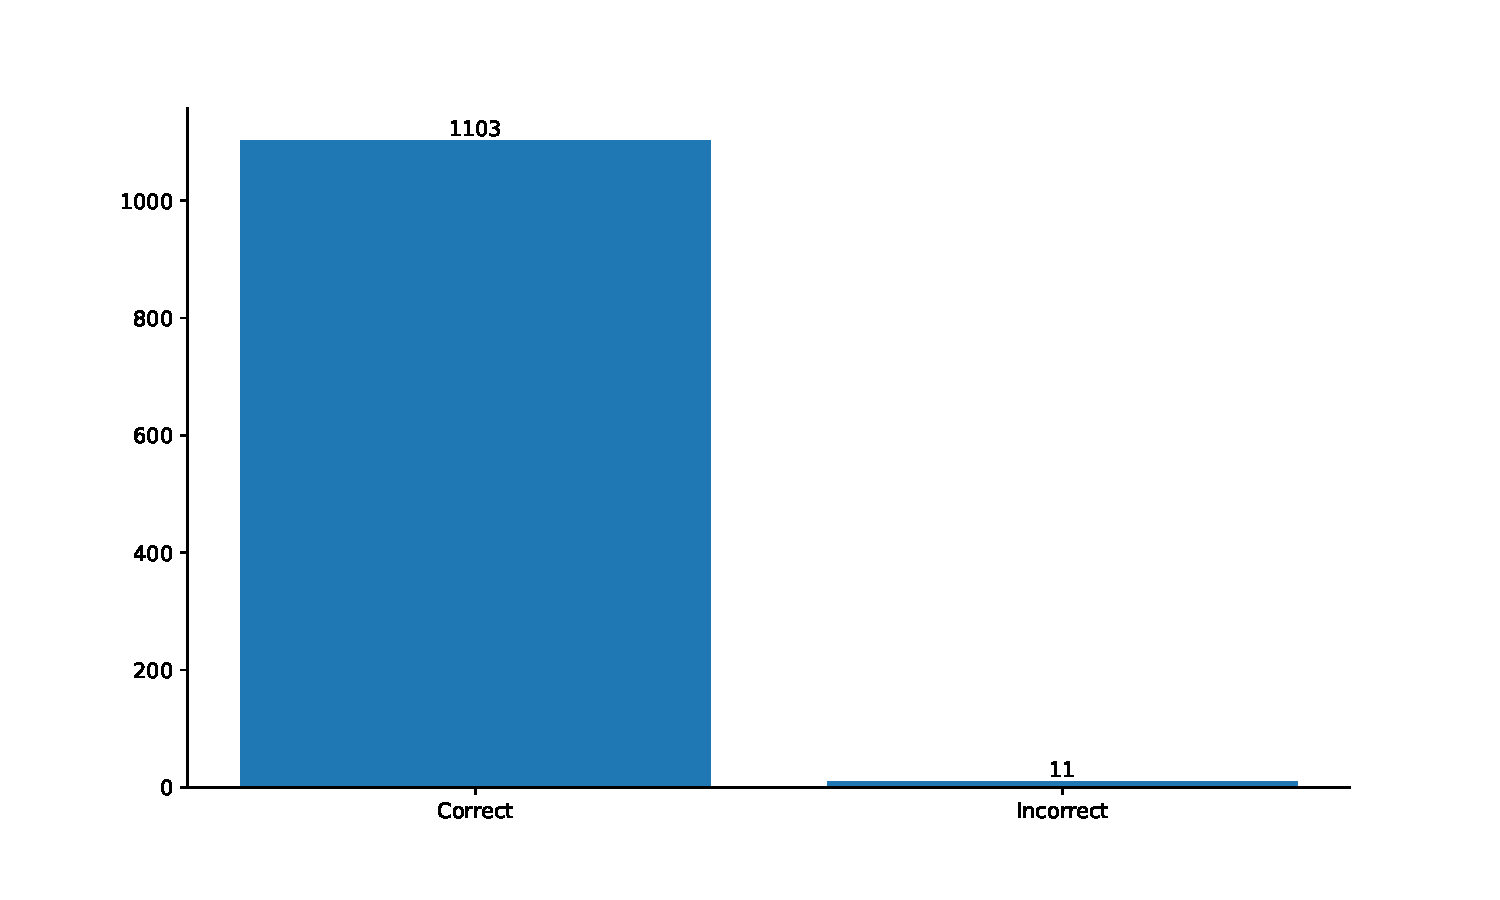
\includegraphics[width=\textwidth]{images/bar_plot.pdf}
  \caption{Results for classifying the test data}
  \label{test-data-result}
\end{figure}

\subsection{Strength and limitations}
Hm let's see if we keep this section

\subsection{Other interesting findings}
I will try to analyze which messages are incorrectly classified.

\section{Conclusion}
This section concludes this report on our implementation of a Naive Bayes spam filter for our course \textit{Natural Language Processing}.

\subsection{Further improvements}

\subsection{Summary}
We want to finish this report with a short summary of our work:

\begin{itemize}
	\item We want to implement a spam filter based on the Naive Bayes algorithm to detect whether a message is spam or ham
	\item Our algorithm uses multinomial Naive Bayes
	\item Dataset consists of spam and ham SMS messages
	\item 
\end{itemize}

